\documentclass[11pt]{article}
%%%%%%%%%%%%%%%%%%%%%%%%%%%%%%%%%%%%%%%%%%%%%%%%%%%%%%%%%%%%%%%
% DO NOT EDIT THIS FILE UNLESS YOU KNOW WHAT YOU ARE DOING!!! %
%%%%%%%%%%%%%%%%%%%%%%%%%%%%%%%%%%%%%%%%%%%%%%%%%%%%%%%%%%%%%%%

\usepackage[]{authblk}
\usepackage{graphicx}
\usepackage{color}
\usepackage{longtable}
\usepackage{hanging}
\usepackage{indentfirst}
\usepackage{setspace}
\usepackage{enumitem}
\usepackage{verbatim}
\usepackage{upgreek}
\usepackage{framed}
\usepackage{textcomp}
\usepackage{url}
\usepackage{soul}
\usepackage{amsmath, amsfonts,amssymb,mathrsfs}
\usepackage{fancyhdr}
\usepackage[compact]{titlesec}
\usepackage[T1]{fontenc}
\usepackage{lmodern}

\usepackage[backend=bibtex,hyperref=true,citestyle=authoryear,bibstyle=authortitle,firstinits=true,terseinits=true,doi=false,url=false,eprint=false,maxbibnames=10,maxcitenames=2]{biblatex}
\DeclareCiteCommand{\cite}
  {\usebibmacro{prenote}}
  {\usebibmacro{citeindex}%
   \printtext[bibhyperref]{\usebibmacro{cite}}}
  {\multicitedelim}
  {\usebibmacro{postnote}}

\DeclareCiteCommand*{\cite}
  {\usebibmacro{prenote}}
  {\usebibmacro{citeindex}%
   \printtext[bibhyperref]{\usebibmacro{citeyear}}}
  {\multicitedelim}
  {\usebibmacro{postnote}}

\DeclareCiteCommand{\parencite}[\mkbibparens]
  {\usebibmacro{prenote}}
  {\usebibmacro{citeindex}%
    \printtext[bibhyperref]{\usebibmacro{cite}}}
  {\multicitedelim}
  {\usebibmacro{postnote}}

\DeclareCiteCommand*{\parencite}[\mkbibparens]
  {\usebibmacro{prenote}}
  {\usebibmacro{citeindex}%
    \printtext[bibhyperref]{\usebibmacro{citeyear}}}
  {\multicitedelim}
  {\usebibmacro{postnote}}

\DeclareCiteCommand{\footcite}[\mkbibfootnote]
  {\usebibmacro{prenote}}
  {\usebibmacro{citeindex}%
  \printtext[bibhyperref]{ \usebibmacro{cite}}}
  {\multicitedelim}
  {\usebibmacro{postnote}}

\DeclareCiteCommand{\footcitetext}[\mkbibfootnotetext]
  {\usebibmacro{prenote}}
  {\usebibmacro{citeindex}%
   \printtext[bibhyperref]{\usebibmacro{cite}}}
  {\multicitedelim}
  {\usebibmacro{postnote}}

\DeclareCiteCommand{\textcite}
  {\boolfalse{cbx:parens}}
  {\usebibmacro{citeindex}%
   \printtext[bibhyperref]{\usebibmacro{textcite}}}
  {\ifbool{cbx:parens}
     {\bibcloseparen\global\boolfalse{cbx:parens}}
     {}%
   \multicitedelim}
  {\usebibmacro{textcite:postnote}}

\newcommand{\citep}{\parencite}
\newcommand{\citet}{\textcite}
\defbibheading{relevref}[\refname]{\section*{Relevant References}}

\renewcommand{\postnotedelim}{\iffieldpages{postnote}{\addcolon}{\addcomma\space}} 
\DeclareFieldFormat{postnote}{#1} 

\DeclareFieldFormat[article, inbook, incollection, inproceedings, patent, thesis, unpublished]{title}{#1}
\DeclareFieldFormat[article, inbook, incollection, inproceedings, patent, thesis, unpublished]{journaltitle}{\mkbibemph{#1}\nopunct}
\DeclareFieldFormat[article, inbook, incollection, inproceedings, patent, thesis, unpublished]{volume}{{#1}\addcolon} %puts volume number in parens
%\DeclareFieldFormat[article, inbook, incollection, inproceedings, patent, thesis, unpublished]{year}{\mkbibparens{#1}\nopunct} %puts year in parens

\DeclareFieldFormat[article, incollection, patent, thesis, unpublished]{pages}{{\nopp#1}}

\DeclareFieldFormat{sentencecase}{\MakeSentenceCase{#1}}

\renewbibmacro*{title}{%
  \ifthenelse{\iffieldundef{title}\AND\iffieldundef{subtitle}}
    {}
    {\ifthenelse{\ifentrytype{article}\OR\ifentrytype{inbook}%
      \OR\ifentrytype{incollection}\OR\ifentrytype{inproceedings}%
      \OR\ifentrytype{inreference}}
      {\printtext[title]{%
        \printfield[sentencecase]{title}%
        \setunit{\subtitlepunct}%
        \printfield[sentencecase]{subtitle}}}%
      {\printtext[title]{%
        \printfield[titlecase]{title}%
        \setunit{\subtitlepunct}%
        \printfield[titlecase]{subtitle}}}%
     \newunit}%
  \printfield{titleaddon}}

\DefineBibliographyStrings{english}{% various adjustments to common bib entry strings
urlseen = {Accessed:},% What goes in front of the date a URL was accessed/retrieved etc.
editor = {(Ed)},%Ed – no dot, in brackets
editors = {(Eds)},% Eds – no dot, in brackets
byeditor = {(Ed.)}}% ‘Edited by’ for edited works

\DeclareNameAlias{default}{last-first}

\renewbibmacro{in:}{}

\renewbibmacro{publisher+location+date}{
  \iflistundef{publisher}
    {}
    {\printlist{publisher}%
       {\addcomma\space}%
      \iflistundef{location}
        {}
        {\printlist{location}}%
    }
}

\DeclareBibliographyDriver{article}{%
\usebibmacro{bibindex}%
\usebibmacro{begentry}%
\usebibmacro{author/translator+others}%
\newunit\newblock
\printfield{year}%
\setunit{\labelnamepunct}\newblock
\usebibmacro{title}%
\newunit
\printlist{language}%
\newunit\newblock
\usebibmacro{byauthor}%
\newunit\newblock
\usebibmacro{bytranslator+others}%
\newunit\newblock
\printfield{version}%
\newunit\newblock
%\usebibmacro{in:}% %mit in:
\usebibmacro{journal}%
\newunit\newblock
\printfield{volume}%
\newunit\newblock
\usebibmacro{byeditor+others}%
\newunit\newblock
\usebibmacro{note+pages}%
\newunit\newblock
\iftoggle{bbx:isbn}
{}%
\newunit\newblock
\usebibmacro{doi+eprint+url}%
\newunit\newblock
\usebibmacro{addendum+pubstate}%
\newunit\newblock
\usebibmacro{pageref}%
\usebibmacro{finentry}}

\DeclareBibliographyDriver{inproceedings}{%
\usebibmacro{bibindex}%
\usebibmacro{begentry}%
\usebibmacro{author/translator+others}%
\newunit\newblock
\printfield{year}%
\setunit{\labelnamepunct}\newblock
\usebibmacro{title}%
\newunit
\printlist{language}%
\newunit\newblock
\usebibmacro{byauthor}%
\newunit\newblock
\usebibmacro{bytranslator+others}%
\newunit\newblock
\printfield{version}%
\newunit\newblock
%\usebibmacro{in:}% %mit in:
\usebibmacro{booktitle}%
\newunit\newblock
\printfield{volume}%
\newunit\newblock
\usebibmacro{byeditor+others}%
\newunit\newblock
\usebibmacro{publisher+location+date}%
\newunit\newblock
\usebibmacro{note+pages}%
\newunit\newblock
\usebibmacro{pageref}%
\usebibmacro{finentry}}

\DeclareBibliographyDriver{book}{%
\usebibmacro{bibindex}%
\usebibmacro{begentry}%
\usebibmacro{author/translator+others}%
\newunit\newblock
\printfield{year}%
\setunit{\labelnamepunct}\newblock
\usebibmacro{title}%
\newunit
\printlist{language}%
\newunit\newblock
\usebibmacro{byauthor}%
\newunit\newblock
\usebibmacro{bytranslator+others}%
\newunit\newblock
%\usebibmacro{in:}% %mit in:
\usebibmacro{booktitle}%
\newunit\newblock
\printfield{volume}%
\newunit\newblock
\usebibmacro{publisher+location+date}%
\newunit\newblock
\usebibmacro{note+pages}%
\newunit\newblock
\usebibmacro{pageref}%
\usebibmacro{finentry}}




\setlist{nolistsep}

\setlength{\evensidemargin}{0in}
\setlength{\headheight}{0in}
\setlength{\headsep}{0in}
\setlength{\oddsidemargin}{-0.25in}
\setlength{\paperheight}{11in}
\setlength{\paperwidth}{8.5in}
\setlength{\tabcolsep}{0in}
\setlength{\textheight}{9in}
\setlength{\textwidth}{7in}
\setlength{\topmargin}{0in}
\setlength{\topskip}{0in}
\setlength{\voffset}{0in}
\parskip = 0.15in
\pagestyle{plain}
\setlength{\parindent}{0cm}

\definecolor{citescol}{RGB}{194,101,1}
\definecolor{urlscol}{RGB}{0,150,206}
\definecolor{linkscol}{RGB}{149,0,207}
\definecolor{mycol}{RGB}{25,23,191}
\definecolor{outputcol}{RGB}{34,139,34}
\definecolor{tcol}{RGB}{165,0,14}


\DeclareMathAlphabet{\msfsl}{T1}{cmr}{m}{it}
\DeclareMathAlphabet{\msyf}{OMX}{pcr}{m}{it}
\newcommand{\alf}{\upalpha}
\newcommand{\hilight}[1]{\colorbox{yellow}{#1}}

\newcommand{\levelone}[1]{
\bigskip
\noindent{\LARGE{\textsc{#1}}}
\vspace {0.05in}
}

\newcommand{\leveltwo}[1]{
\bigskip
\noindent{\Large{\textit{#1}}}
\vspace {-1mm}
}

\newcommand{\descriptionhead}[1]{
\noindent{\textcolor{mycol}{\textbf{\textit{#1}}}}\\ \vspace{-7mm}
}

\newcommand{\dhead}[1]{
\noindent{\textbf{\textit{#1 --}}}
}



\newcommand{\exs}[1]{
\vspace{-4mm}
\begin{itemize}
\item #1 \\ \vspace{-8mm}
\end{itemize}
}

\newcommand{\nbo}[1]{{\color{red}{#1}}}


\newcommand{\stepbullet}{\noindent \textbullet \ }
\newcommand{\mi}[1]{\textbf{\textit{#1}}}


\newcommand{\levelthree}[1]{\textit{#1 --}}


%\bibliographystyle{apalike}
%\bibpunct[; ]{(}{)}{;}{a}{,}{;}


\usepackage[breaklinks]{hyperref}
\usepackage[all]{hypcap}
\hypersetup{colorlinks=true,linkcolor=linkscol,citecolor=citescol,urlcolor=urlscol}


\newcommand{\R}{\texttt{R} }
\newcommand{\TESS}{\texttt{TESS}}
\newcommand{\PBD}{\texttt{PBD}}
\newcommand{\DDD}{\texttt{DDD}}
\newcommand{\Laser}{\texttt{laser}}
\newcommand{\TreePar}{\texttt{TreePar}}
\newcommand{\diversitree}{\texttt{diversitree}}
\newcommand{\RevBayes}{\texttt{RevBayes}}
\newcommand{\Rev}{\texttt{Rev}}
\newcommand{\MrBayes}{\texttt{MrBayes}}
\newcommand{\BEAST}{\texttt{BEAST}}
\newcommand{\PhyloBayes}{\texttt{PhyloBayes}}
\newcommand{\PAML}{\texttt{PAML}}

\let\otheriint\iint
\let\iint\relax
\usepackage{ wasysym }

\usepackage{framed}
\usepackage[]{listings}
%\usepackage{fontspec}
\usepackage{placeins}
\usepackage{epstopdf}



\lstset{backgroundcolor=\color[rgb]{0.972,0.972,0.972},
		tabsize=4,
		rulecolor=,
        basicstyle=\scriptsize,
        upquote=true,
        aboveskip={1.5\baselineskip},
        columns=fixed,
        showstringspaces=false,
        extendedchars=true,
        breaklines=true,
        prebreak = \raisebox{0ex}[0ex][0ex]{\ensuremath{\hookleftarrow}},
        frame=single,
        showtabs=false,
        showspaces=false,
        showstringspaces=false,
        identifierstyle=\ttfamily,
        keywordstyle=\color[rgb]{0,0,1},
        commentstyle=\color[rgb]{0.133,0.545,0.133},
        stringstyle=\color[rgb]{0.627,0.126,0.941}
}

\definecolor{shadecolor}{RGB}{194,225,255}

\setlength{\tabcolsep}{5pt}
\setlength{\topmargin}{-0.4in}
\setlength{\headheight}{14.5pt}
\pagestyle{fancy}

\newcommand{\taha}[1]{{\textcolor{red}{[TAH comment: #1]}}} % TAH comment

\titlespacing{\section}{0pt}{*0}{*0}
\titlespacing{\subsection}{0pt}{*0}{*0}
\titlespacing{\subsubsection}{0pt}{*0}{*0}

\titleformat{\section}
  {\normalfont\Large\bfseries\color{mycol}}
  {\thesection}{1em}{}

\titleformat{\subsection}
  {\normalfont\large\bfseries\color{mycol}}
  {\thesubsection}{1em}{}

\titleformat{\subsubsection}
  {\normalfont\bfseries\color{mycol}}
  {\thesubsubsection}{1em}{}

% command for MrBayes command-line step
\newcommand{\cl}[1]{{\texttt{\textbf{#1}}}}

\newcommand{\colx}[1]{{\textcolor{tcol}{#1}}}

\newcommand{\mbcl}[1]{\exs{\cl{MrBayes > {#1}}}}

\newcommand{\rbprmt}{RevBayes > } 
\newcommand{\rbcl}[1]{\exs{\cl{\rbprmt{#1}}}}
\newcommand{\rbout}[1]{\exs{\cl{\textcolor{outputcol}{#1}}}}
\newcommand{\rbdn}{{\Large \symbol{126}}} % This makes a copy/pasteable tilde
\newcommand{\rbclml}[1]{\exs{\cl{\ \ \ \ \ \ \ \ \ \ \ {#1}}}}

% text box settings
% requires compiling w/ XeLaTeX
%\newfontfamily\listingsfont[Scale=1.0]{Courier New}
%\lstset{basicstyle=\listingsfont, columns=texcl}
%\defaultfontfeatures{Mapping=tex-text}


\makeatletter
\lst@CCPutMacro\lst@ProcessOther {"2D}{\lst@ttfamily{-{}}{-{}}}
\@empty\z@\@empty
\makeatother


\usepackage{tikz}

\setlength{\topmargin}{-0.4in}
\setlength{\headheight}{14.5pt}
\pagestyle{fancy}

\usepackage[breaklinks]{hyperref}
\usepackage[all]{hypcap}
\hypersetup{colorlinks=true,linkcolor=linkscol,citecolor=citescol,urlcolor=urlscol}

\definecolor{lg}{gray}{0.75}
\def\gcirc{{%
    \setbox0\hbox{$\fullmoon$}%
    \rlap{\hbox to \wd0{\hss{$\textcolor{lg}{\newmoon}$}\hss}}\box0
}}



% Add your bibtex library here
\addbibresource{refs.bib}


%%%%%%%%%%%%%%%%%%%%
% Do NOT edit this %
%%%%%%%%%%%%%%%%%%%%
\begin{document}
\renewcommand{\headrulewidth}{0.5pt}
\headsep = 20pt
\lhead{ }
\rhead{\textsc {BEAST v2 Tutorial}}
\thispagestyle{plain}


%%%%%%%%%%%%%%%%%%
% Tutorial title %
%%%%%%%%%%%%%%%%%%
\begin{center}

	% Enter the name of your tutorial here
	\textbf{\LARGE Species Trees and Species Delimitation with SNAPPER}\\\vspace{2mm}

	% Enter a short description of your tutorial here
	\textbf{\textcolor{mycol}{\Large Analyzing SNP or AFLP data}}\\

	\vspace{4mm}

	% Enter the names of all the authors here
	{\Large {\em Adam Leaché, Remco Bouckaert}}
\end{center}


%%%%%%%%%%%%%%%%%
% Tutorial body %
%%%%%%%%%%%%%%%%%

\hypertarget{background}{%
\section{Background}\label{background}}

This tutorial will help you become familiar with conducting species tree inference and species delimitation in a Bayesian framework using biallelic markers (AFLP or SNP data) using the package \verb8SNAPPER8 in BEAST2.

Coalescent methods for estimating species trees typically rely on estimating a gene tree for each locus. Combining hundreds or thousands of gene trees into a coalescent-based species tree inference framework presents some serious computational challenges. SNAPP is a method for estimating species trees that does not require gene trees \cite{Bryant2012}, and SNAPPER \cite{stoltz2021bayesian} is a fast and good approximation to SNAPP.
This approach has been applied to the problem of species delimitation \citep{Leache14}. The species tree estimation method SNAPPER \citep{Bryant2012,stoltz2021bayesian} estimates species trees directly from biallelic markers (e.g., SNP or AFLP data), which bypasses the necessity of having to explicitly integrate or sample the gene trees at each locus. The method works by estimating the probability of allele frequency change across ancestor/descendent nodes. The result is a posterior distribution for the species tree, species divergence times, and effective population sizes, all obtained without the estimation of gene trees. The method works well for relatively small numbers of species (minimum = 2; maximum is probably near 20 due to computational constraints). Multiple alleles should be sampled for each species.

Species delimitation using genetic data and coalescent methods are increasing in popularity for good reasons \citep{Fujita2012}. Comparing candidate species delimitation models that contain different numbers of species, or different allocations of populations to species, is relatively easy in a Bayesian framework. The general approach is to estimate the marginal likelihood \citep{baele12} of each competing species delimitation model, rank models by marginal likelihood, and use Bayes factors \citep{kass95} to assess support for model rankings. This approach, called Bayes factor delimitation (BFD), was first implemented by \citet{Grummer13} with DNA sequences in the program *BEAST. The approach was modified to work with SNP data (BFD*) \citep{Leache14} using the  SNAPPER model.

BFD* estimates the species tree and evaluates the species delimitation model at the same time, while allowing the user to compare models that contain different numbers of species and different assignments of samples to species. This is useful when the goal is to compare predefined species delimitation models or competing taxonomies. However, one drawback is that the user needs to predefine the number of species and sample assignments. This prevents the method from searching among all possible species assignments, an obvious disadvantage for studies aiming to discover cryptic diversity. Another major limitation is that the method does not explicitly consider gene flow, isolation by distance, selection, or several other important biological processes; however, these limitations are shared by many current methods. For example, failing to sample admixed populations often favours models containing more species, whereas including admixed populations will support more models containing fewer species. Distinguishing among these problematic scenarios requires paying close attention to both sample selection and prior settings. Finally, when evaluating results, remember to consider other aspects of the biology, ecology, and geography of ``species'' before jumping to conclusions. \clearpage

\hypertarget{programs-used-in-this-exercise}{%
\section{Programs used in this
Exercise}\label{programs-used-in-this-exercise}}

\hypertarget{beast2---bayesian-evolutionary-analysis-sampling-trees-2}{%
\subsubsection{BEAST2 - Bayesian Evolutionary Analysis Sampling Trees
2}\label{beast2---bayesian-evolutionary-analysis-sampling-trees-2}}

BEAST2 is a free software package for Bayesian evolutionary analysis of
molecular sequences using MCMC and strictly oriented toward inference
using rooted, time-measured phylogenetic trees \citep{Bouckaert2014}.
This tutorial uses BEAST2 version 2.7.4.

\hypertarget{beauti-bayesian-evolutionary-analysis-utility}{%
\subsubsection{BEAUti -- Bayesian Evolutionary Analysis
Utility}\label{beauti-bayesian-evolutionary-analysis-utility}}

BEAUti is a utility program with a graphical user interface for creating
BEAST2 input files, which are written in XML. The eXtensible Markup
Language (XML) is a general-purpose markup language, which allows for
the combination of text and additional information. The use of the XML
makes analysis specification very flexible and readable by both the
program and people. The XML file specifies all the components of the
analysis, including sequences, node calibrations, models, priors, output
file names.

\hypertarget{treeannotator}{%
\subsubsection{TreeAnnotator}\label{treeannotator}}

TreeAnnotator is used to summarize the posterior sample of trees to
produce a maximum clade credibility tree and summarize the posterior
estimates of other parameters that can be easily visualized on the tree
(e.g.~node height). This program is also useful for comparing a specific
tree topology and branching times to the set of trees sampled in the
MCMC analysis.

\hypertarget{tracer}{%
\subsubsection{Tracer}\label{tracer}}

Tracer is used for assessing and summarizing the posterior estimates of
the various parameters sampled by the Markov Chain. This program can be
used for visual inspection and assessment of convergence and it also
calculates 95\% credible intervals (which approximate the 95\% highest
posterior density intervals) and effective sample sizes (ESS) of
parameters. Contrary to the other software in this section, Tracer is
not distributed with BEAST2 and needs to be downloaded separately
\href{http://beast.community/tracer}{here}. \clearpage

\hypertarget{practical-species-delimitation}{%
\section{Practical: species delimitation}\label{practical-species-delimitation}}

\hypertarget{dataset}{%
\subsection{Dataset}\label{dataset}}

The dataset used in this tutorial contains SNP data for geckos in the \textit{Hemidactylus fasciatus} species complex. Details on how the data were collected are 
provided in \citep{Leache14}. For this tutorial, we will use a data matrix containing 129 SNPs that is also available for download on \href{http://datadryad.org/resource/doi:10.5061/dryad.r55fb}{Dryad}. Allopatric divergence seems to be the primary mechanism causing speciation in this group. These geckos are restricted to rainforest habitats, and their distributions match those of the major blocks of rainforest in West and Central Africa (Figure \ref{fig:map}). 

For this species delimitation example, we will test models based on historical connections between adjacent rainforest blocks. These models differ in the number of species, and how samples are assigned to species. The base model has four species (Figure \ref{fig:map}a). The alternative models are grouped into three classes: (1) lumping: populations are collapsed into the same species, (2) splitting: populations are partitioned into separate species, (3) reassigning: population(s) are allocated into a different species.

\begin{figure}[htbp]
    \centering
    \fbox{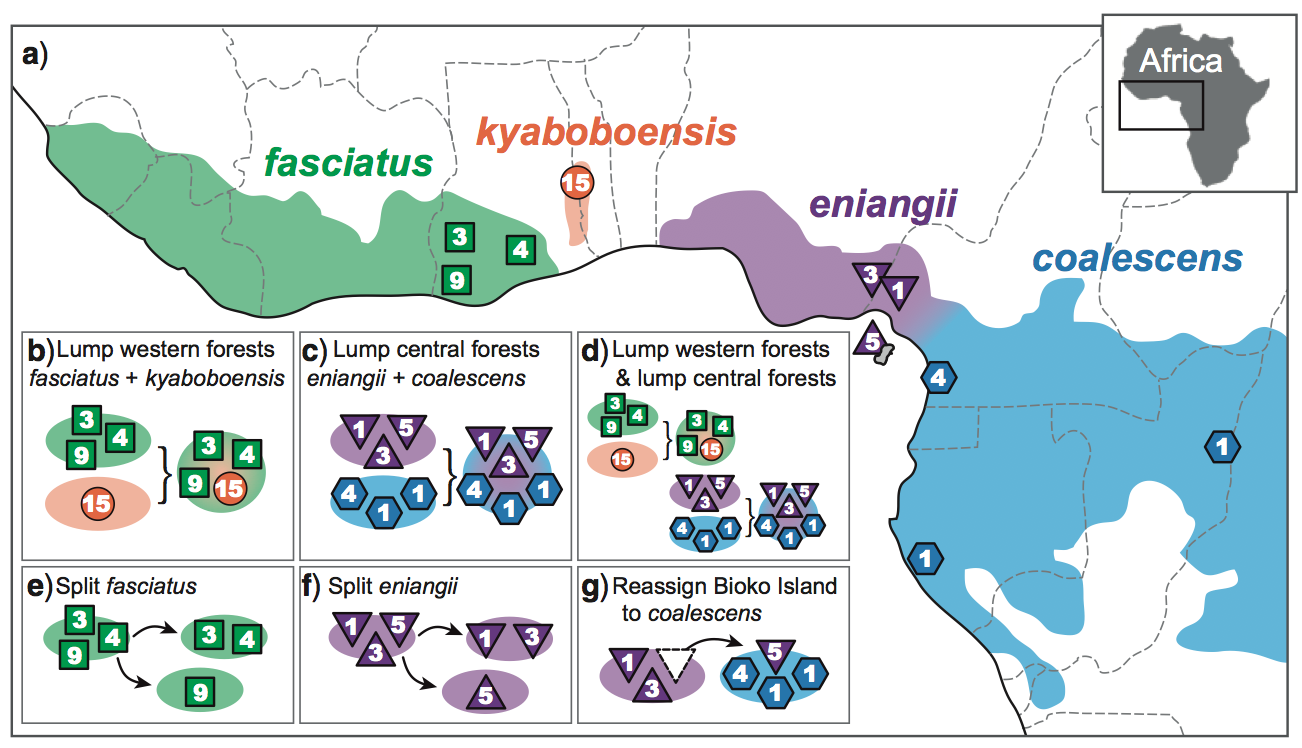
\includegraphics[width=0.8\textwidth]{figures/map.png}}
    \caption{Geographic sampling of geckos (numbers in symbols indicate sample sizes). Starting taxonomy is shown in (a). BFD* is used to test the alternative species delimitation models outlined in (b) -- (g)
    and (s) which combines (b) and (g).}
    \label{fig:map}
\end{figure}
    
The gecko SNP data is in binary format (necessary for SNAPPER). If you are unsure of how to convert your own SNP data from nucleotide to binary format, please read the documentation \href{http://beast2.org/tutorials/}{A rough guide to SNAPP} (Section 4. Preparing Input File). You can find scripts for converting SNP data into SNAPPER input format at the phrynomics project site at \href{https://github.com/bbanbury/phrynomics}{GitHub}. You can also find help at the BEAST2 \href{https://groups.google.com/forum/?fromgroups\#!forum/beast-users}{google users group}.


\hypertarget{setting-up-the-xml-file}{%
\subsection{Setting up the XML file}\label{setting-up-the-xml-file}}

This section will demonstrate how to create an XML configuration file using BEAUti, which will then be used to run the analysis in BEAST2.


\hypertarget{package-installation}{%
\subsubsection{Package installation}\label{package-installation}}

We need to install additional packages to run this analysis.

\begin{framed}
    Open the \textbf{BEAST2 Package Manager} by navigating to \textbf{File \textgreater{} Manage Packages}. (Figure \ref{packageManage1})
\end{framed}

\begin{figure}
    \centering
    \fbox{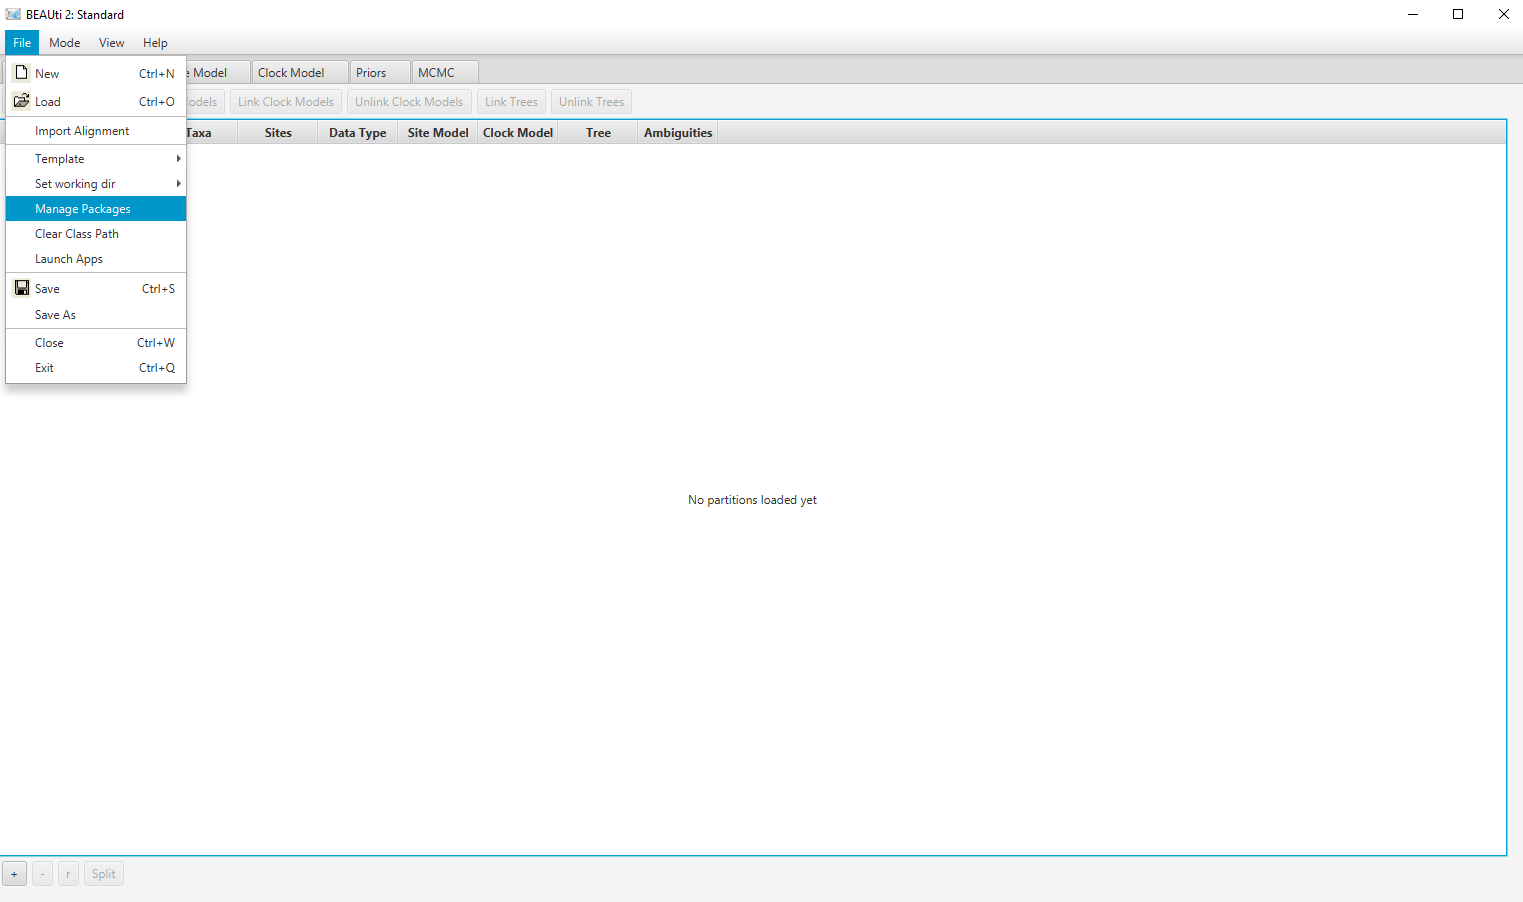
\includegraphics[width=0.750000\textwidth]{figures/package_manager.png}}
    \caption{Finding the BEAST2 package manager.}
    \label{packageManage1}
\end{figure}

\begin{framed}
    Install the \textbf{SNAPPER} and \textbf{Model\_Selection} packages by selecting them and clicking the
    \textbf{Install/Upgrade} button. (Figure \ref{fig:beauti-manage-packages})
\end{framed}

\begin{figure}[htbp]
    \centering
    \fbox{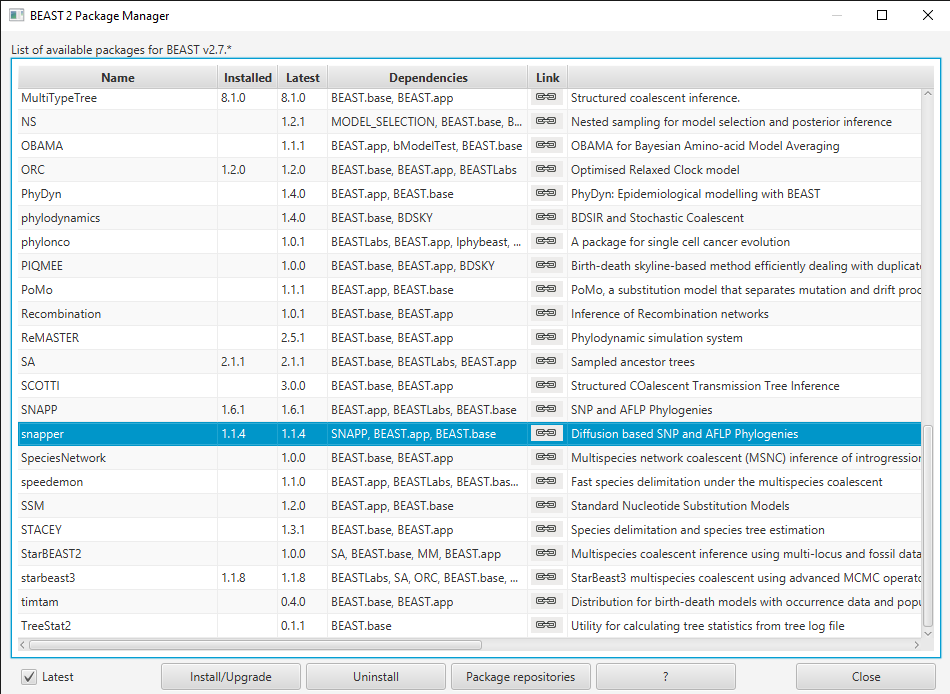
\includegraphics[width=0.7\textwidth]{figures/beauti-manage-packages.png}}
    \caption{BEAUti package manager for BEAST2.}
    \label{fig:beauti-manage-packages}
\end{figure}

Since \textbf{SNAPPER} depends on the \textbf{SNAPP} package and \textbf{Model\_Selection} on the \textbf{BEASTLabs} package, these packages will be automatically installed as well. BEAUti needs to be restarted for the newly installed packages to be loaded properly.

\begin{framed}
    Close the \textbf{BEAST2 Package Manager} and \textbf{\emph{restart}} BEAUti to fully load the new packages.
\end{framed}

\hypertarget{setting-the-template}{%
\subsubsection{Setting the template}\label{setting-the-template}}

We need to tell BEAUti that we are setting up a SNAPPER analysis, which will change the menu options and allow us to import SNP data.

\begin{framed}
    Select the template by using the drop-down menu \textbf{File \textgreater{} Template \textgreater{} SNAPPER}.
    This should change the appearance of the BEAUti window to look something like Figure~\ref{fig:beauti-SNAPPER}.
\end{framed}

\begin{figure}[htbp]
    \centering
    \fbox{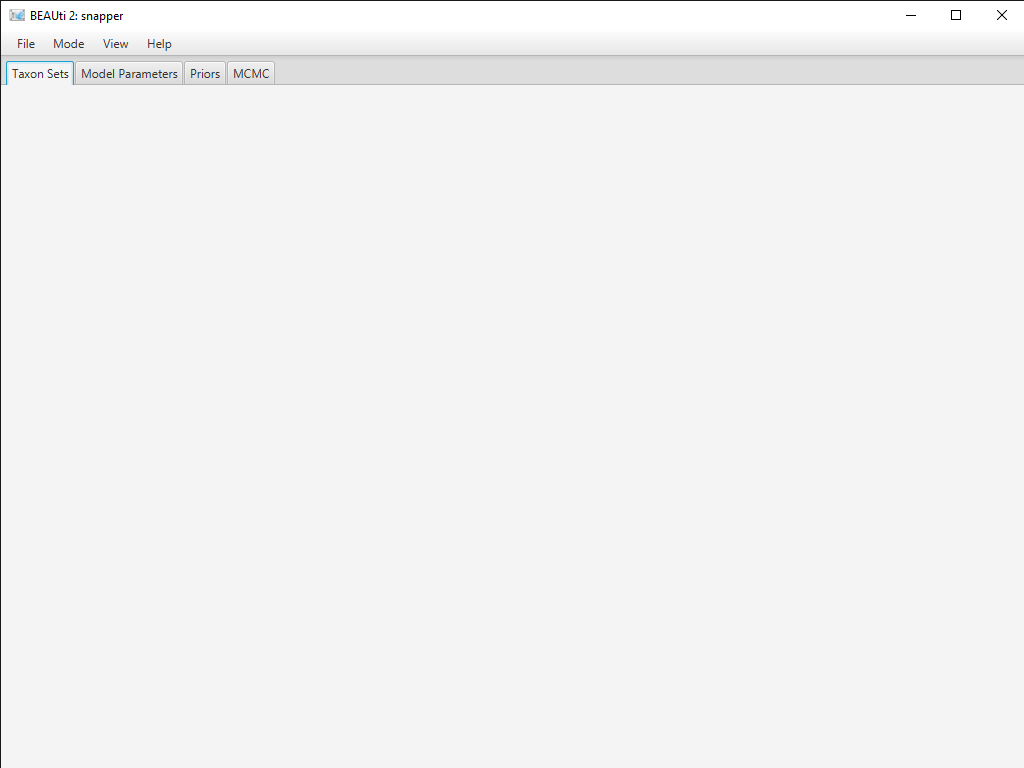
\includegraphics[width=0.7\textwidth]{figures/beauti-snapper.png}}
    \caption{BEAUti window after importing the SNAPPER template. Notice that the menu tabs have changed.}
    \label{fig:beauti-SNAPPER}
\end{figure}

\subsubsection{Importing the SNP data}

\begin{framed}
    Import the SNP data (the {\bf hemi129.nex} file)
    using the drop-down menu \textbf{File \textgreater{} Import Alignment}.\footnote{For the SNAPP tutorial, there is a smaller version of the {\bf hemi129.nex} file called {\bf smallhemi129.nex}. If you load the full data set from {\bf hemi129.nex} with SnAPP you might not finish this tutorial in the allocated time frame. However, the runtime of SNAPPER is not sensitive to the number of sequences per species, just the number of species and length of sequences.}
\end{framed}

Once the data are successfully loaded into BEAUti you should see a list of the 
samples included in the data file (Figure~\ref{fig:beauti-data-imported}.)

\begin{figure}[htbp]
    \centering
    \fbox{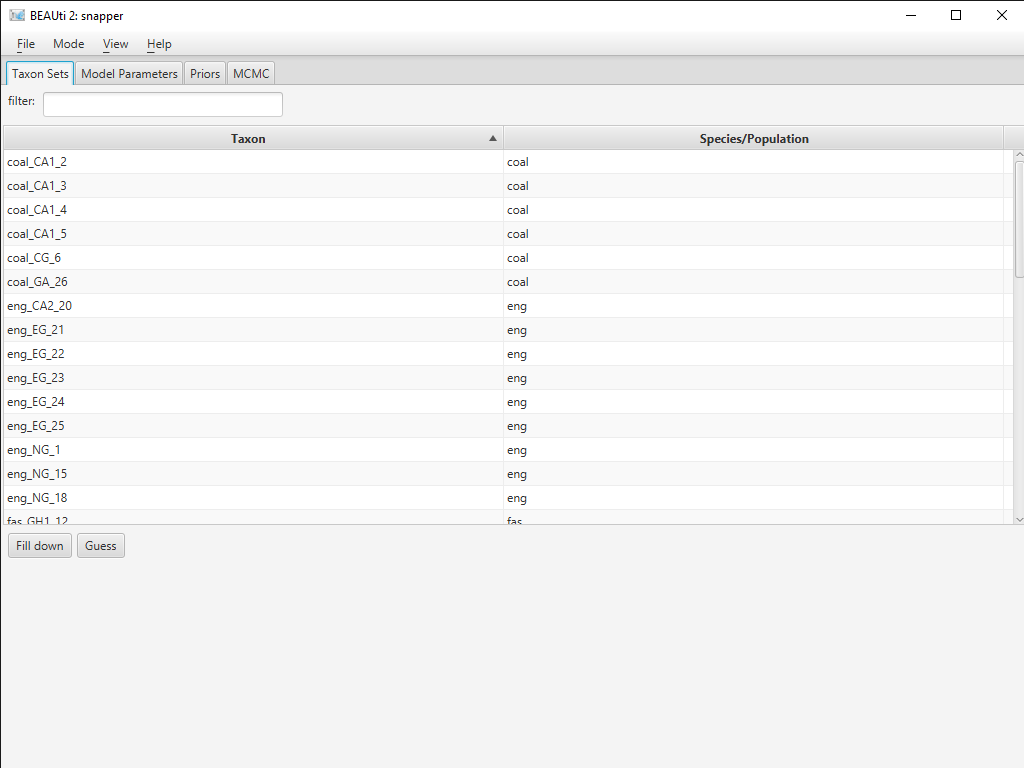
\includegraphics[width=0.8\textwidth]{figures/beauti-data-imported.png}}
    \caption{The data successfully loaded by BEAUti.}
    \label{fig:beauti-data-imported}
\end{figure}

\subsubsection{Defining species}
There are several ways to designate species assignments. You can automatically 
designate species names using the names already 
present in the data files. The species names can be pre-defined this way by including a ``delimiter'' that 
allows the species name to be parsed from the rest of the sequence name. The gecko data 
file uses an underscore ``\_'' to separate
the species name (on the left) from the rest of the sequence name (on the right) as follows:\\
\\
\texttt{eng\_NG\_1}\\ 	
\texttt{coal\_CA1\_2}\\	
\texttt{coal\_CA1\_3}\\
\texttt{coal\_CA1\_4}\\	
\texttt{coal\_CA1\_5}\\	
\texttt{coal\_CG\_6}\\	
\texttt{kya\_GH3\_7}\\	
\texttt{kya\_GH3\_8}\\	
\texttt{\ldots}\\
\\
Other options for assigning species names are available using the ``Guess'' button. 

\begin{framed}
    Open the guessing menu by clicking on \textbf{Guess} button.
    The screen should look similar to Figure~\ref{fig:beauti-guess-trait}.
\end{framed}
    
How many samples should you include? More samples give more accurate estimates and has not computation cost for SNAPPER (unlike SNAPP, which is very sensitive to the number of samples), so the more samples the better.
Keep in mind that the number of species slows down SNAPPER much more than the number of SNPs.
If you have too many species and the analysis rusn unbearably slow, you might sub-sample the number of species.

\begin{figure}[htbp]
    \centering
    \fbox{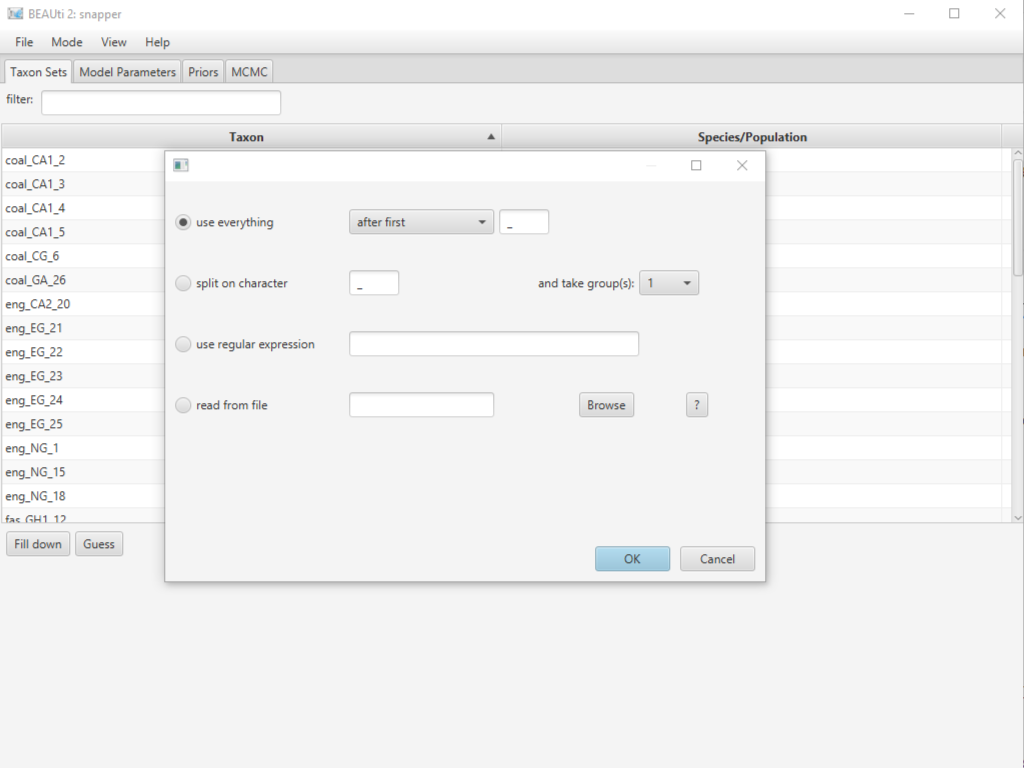
\includegraphics[width=0.8\textwidth]{figures/beauti-guess-trait.png}}
    \caption{The species assignment options that appears after you select the ``Guess' button.}
    \label{fig:beauti-guess-trait}
\end{figure}

You can import a custom mapping file that links each sample to a species using the ``read from file'' option.

\begin{framed}
    Click the ``Ok'' button to return to the \textbf{Taxon Sets} window. Make sure that each Taxon has a Species/Population name.    
\end{framed}

\subsubsection{Setting the model parameters}

Next, we set up our model under the \textbf{Model Parameters} tab.

Be sure to read the documentation \href{http://www.beast2.org/tutorials}{A rough guide to SNAPP} to learn more about the model options\footnote{For SNAPP, the mutation rates U and V representing instantaneous rate of mutating from the 0 allele to the 1 allele and from 1 to 0 respectively are included in the model. However, keeping U and V equal to 1 seems more appropriate, so these parameters are hidden in BEAUti for the SNAPPER model.}. Briefly, the main parameter of interest is the {\tt Coalescent Rate} which determines the population size parameter with one value for each node in the tree.

\textit{Recommendations:}  %Set mutation rates u and v = 1 and do not sample. Alternatively, you can click the {\bf ``Calc mutation rates''} button to get a direct estimate of u and v. Either way, you typically do not have to estimate these parameters during the MCMC. 

``Coalescent Rate'': check the ``estimate`` box. If you do not sample, then you assume that all population sizes are the same, which is unrealistic. The coalescent rate is 2/theta, and the number is simply the starting value used to initialise the analysis. %Do not confuse the coalescent rate with the theta prior. 
%The theta prior is described in detail in the next section.

``N'' is the dimension of Chebyshef functions used for approximating the SNAPP tree likelihood. N should be power of 2 plus 1 (e.g. 33, 17, 65). Higher values are more accurate but slower.

The ``Non-polymorphic'' checkbox is used in cases where invariant sites have been included in the data. The likelihood calculations are 
different if SNAPPER assumes that all constant sites have been removed. If you are using a typical SNP dataset that only includes variable sites, then make sure that the box is not checked.

The ``Mutation Only At Root'' checkbox indicates a conditioning on zero mutations, except at root (default false). As a result, all gene 
trees will coalesce in the root only, and never in any of the branches. This option allows you to emulate the model used by \citet{nielsen1998} and \citet{roychoudhury2008}.
    
The ``Use Log Likelihood Correction'' checkbox is for calculating corrected likelihood values for Bayes factor test of different species assignments (the calculation is almost instantaneous, and it will not slow down your analysis).

When the ``Use beta root prior'' checkbox is checked, instead of using a uniform prior for allele frequencies at the root, a beta root prior is used.


Following these recommendations, the only change we need to make here is to tell BEAUti that our alignment is made of polymorphic sites only.

\begin{framed}
    Uncheck the \textbf{Non-polymorphic} checkbox.
\end{framed}

The final setup will appear as in Figure~\ref{fig:beauti-model}.

\begin{figure}[ht]
    \centering
    \fbox{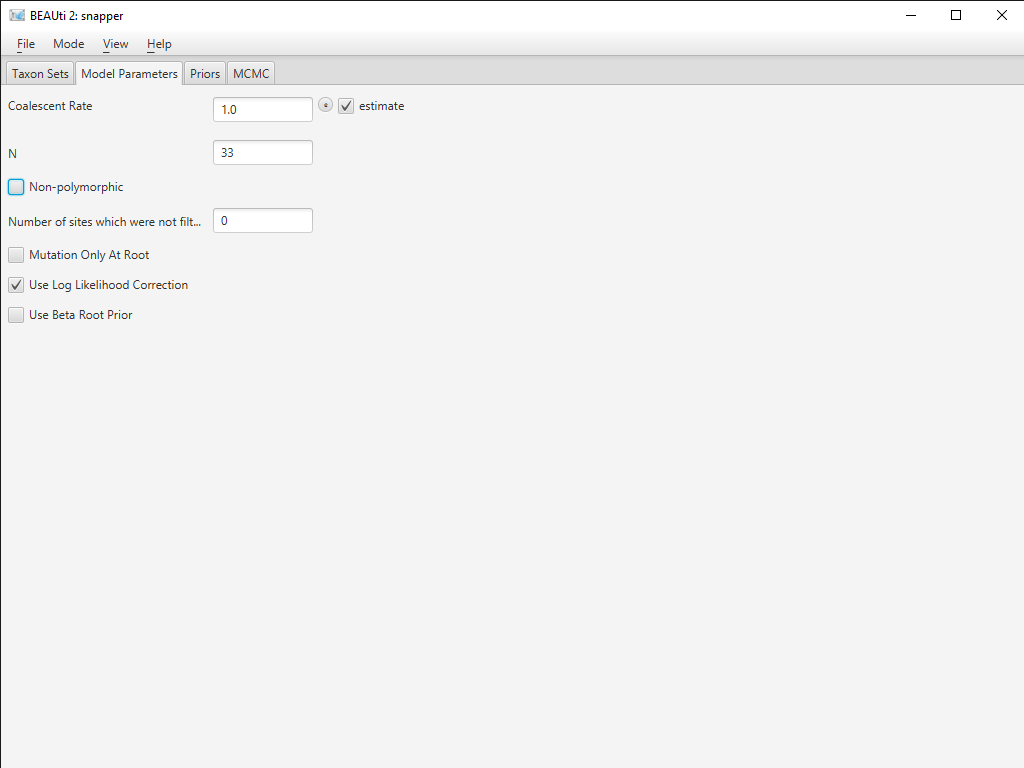
\includegraphics[width=0.8\textwidth]{figures/beauti-model-parameters.png}}
    \caption{The SNAPPER model options.}
    \label{fig:beauti-model}
\end{figure}
    
\subsubsection{Defining the priors}

Next, we move to the \textbf{Prior} tab and specify the priors. Again, read the 
documentation \href{http://www.beast2.org/tutorials}{A rough guide to SNAPP} 
to learn more about these priors. It is important to be aware of the biological meaning of these priors. 
One problem with SNAPPER (and BEAST2 in general) is that it is deceptively easy to set up an analysis using default options. 

The default priors are
\begin{itemize}
\item for the tree, a Yule prior representing a pure birth process with birth rate parameter {$\lambda$}.
\item a {\bf terrible} uniform prior with range 0 to $+\infty$ for the birth rate {$\lambda$}.
\item a gamma prior with shape=2, scale=2 for the coalescent rates.
\end{itemize}

SNAPPER by default uses a Yule prior for the species tree and branch lengths on the species tree. This prior has a single parameter, {$\lambda$} (Lambda), representing the speciation rate. This rate, in turn, determines the (prior) expected height of the species tree. The higher the speciation rate, the higher the probability of supporting more species during species delimitation.

The default prior on {$\lambda$} can seem non-informative, allowing the data to drive the analysis instead of prior information. However, it is an improper prior. A proper prior is a prior that when integrating over its range sums to 1. Since the uniform prior has infinite bounds, the integral over the range does not do that. The prior can be made proper by defining finite upper and lower bounds.\footnote{The 1/X prior is another prior that is not proper and therefore not recommended.} For estimating the marginal likelihood using path sampling, ``proper'' priors are required. In addition this prior puts too much weight on very high and unrealistic values of the birth rate.

So do we set a prior on the birth rate? The trees that come out of SNAPPER are not time calibrated, thus the branch lengths should be interpreted in units of expected substitutions per site. Translating this into time requires an assumption about the substitution rate. See the Rough Guide to SNAPP for further details and an equation for calculating Lambda. Using a useful script written by Jamie Oaks, called \href{https://github.com/joaks1/pyule}{pyule}, you can calculate an appropriate lambda value based on prior information about the number of species, and the height of the species tree in expected substitutions per site. If sequence data are available, then you can approximate the height of the species tree obtained by calculating the maximum observed divergence between any pair of taxa divided by two (height = max divergence/2).

Table \ref{tab:lambda_values} provides some suggestions for good Lambda values across a range of expected substitutions per site from root to tip (up to 20\% sequence divergence from root to any tip), and for relatively small species trees (up to 20 species). In general, different Lambda settings do not influence the results too much, since in most cases the data will dominate. 

\begin{table}[ht]
    \tabcolsep=0.4cm
    \begin{tabular}{rrcccccc}
    \hline
            &    & \multicolumn{6}{c}{Species tree height (expected substitutions per site)}     \\
                            &    	& 0.001 	& 0.005 	& 0.01 	& 0.05  	& 0.10 	&0.2\\
                            &    	&  (0.1\%)	&  (0.5\%) &  (1\%) 	&  (5\%)  	& (10\%)  	& (20\%)\\ \hline
                            & 2 	& 500	& 100 	& 50 		& 10 		& 5 		& 0.2\\
    Number of species 	& 5	& 1283 	& 257 	& 128 	& 26 		& 13 		& 6\\
                            & 10	& 1928 	& 386 	& 193 	& 39 		& 19 		& 10\\
                            & 15	&  2318	&  464	&  232	& 46		& 23		& 12\\
                            & 20	&  2598	&  520	&  260	& 52 		& 26 		& 13\\\hline
    \end{tabular}
    \caption{Lambda prior settings across a range of species tree heights (in expected substitutions per site) and sizes (number of species).}
    \label{tab:lambda_values}
\end{table}

In this case, we are going to set a gamma prior with a broad distribution, for example, alpha = 2 and beta = 200. Note that the mean of the gamma distribution for Lambda is calculated as alpha*beta when mode is 'ShapeScale' (rather than alpha/beta when mode='ShapeRate'). If there is prior information about the number of expected substitutions, then this can be used to set up the prior. In general, you should try setting the mean of the gamma distribution to be somewhere in the middle of the extreme lambda values (shown in Table 1) that apply to your study system.

\begin{framed}
    In the \textbf{Priors} tab, open the dropdown menu next to the \textbf{birthRate} parameter, and change the distribution type from \textbf{Uniform} to \textbf{Gamma}.
    Click on the arrow next to \textbf{birthRate} to open the prior details and check that \textbf{alpha} and \textbf{beta} are set to \textbf{2.0}.
    The prior set up should look like Figure \ref{fig:beauti-prior}.
\end{framed}

\begin{figure}[ht]
    \centering
    \fbox{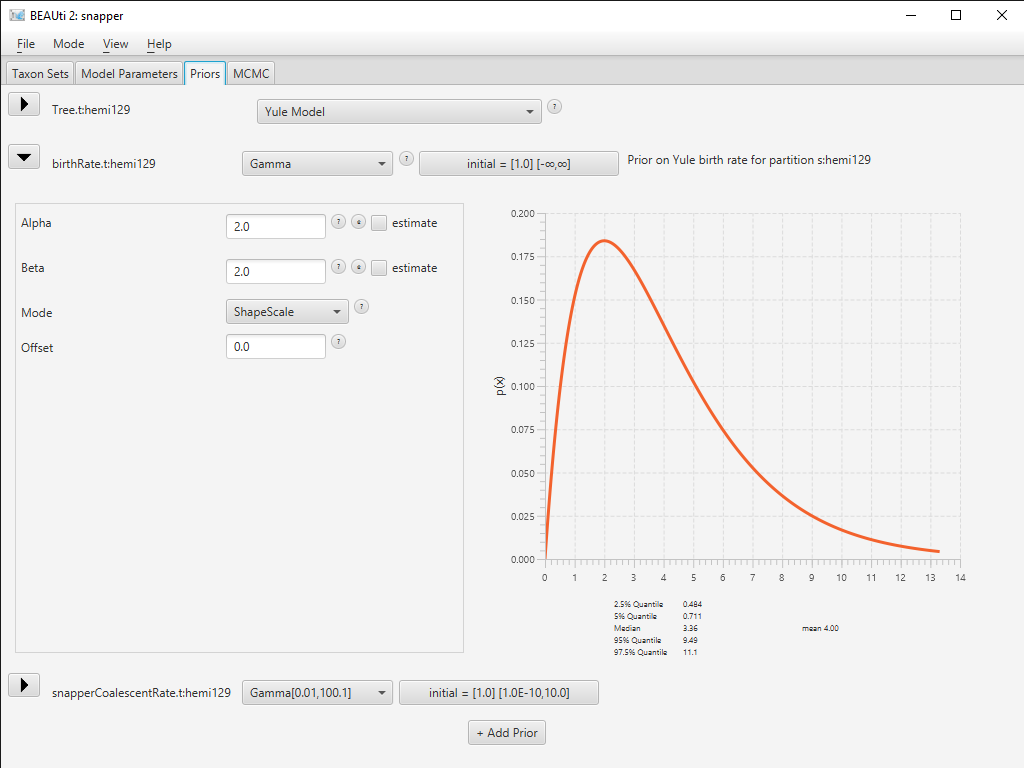
\includegraphics[width=0.8\textwidth]{figures/beauti-prior.png}}
    \caption{The prior settings: using a gamma prior for the birth rate.}
    \label{fig:beauti-prior}
\end{figure}  

Figure \ref{fig:lambda_comparison} shows a comparison of two different options for setting lambda: using a fixed value (lambda = 5) versus assigning a broad gamma prior as we did. In this case, tree height estimates are similar using either a fixed lambda or a gamma distribution. 

\begin{figure}[ht]
    \centering
    \fbox{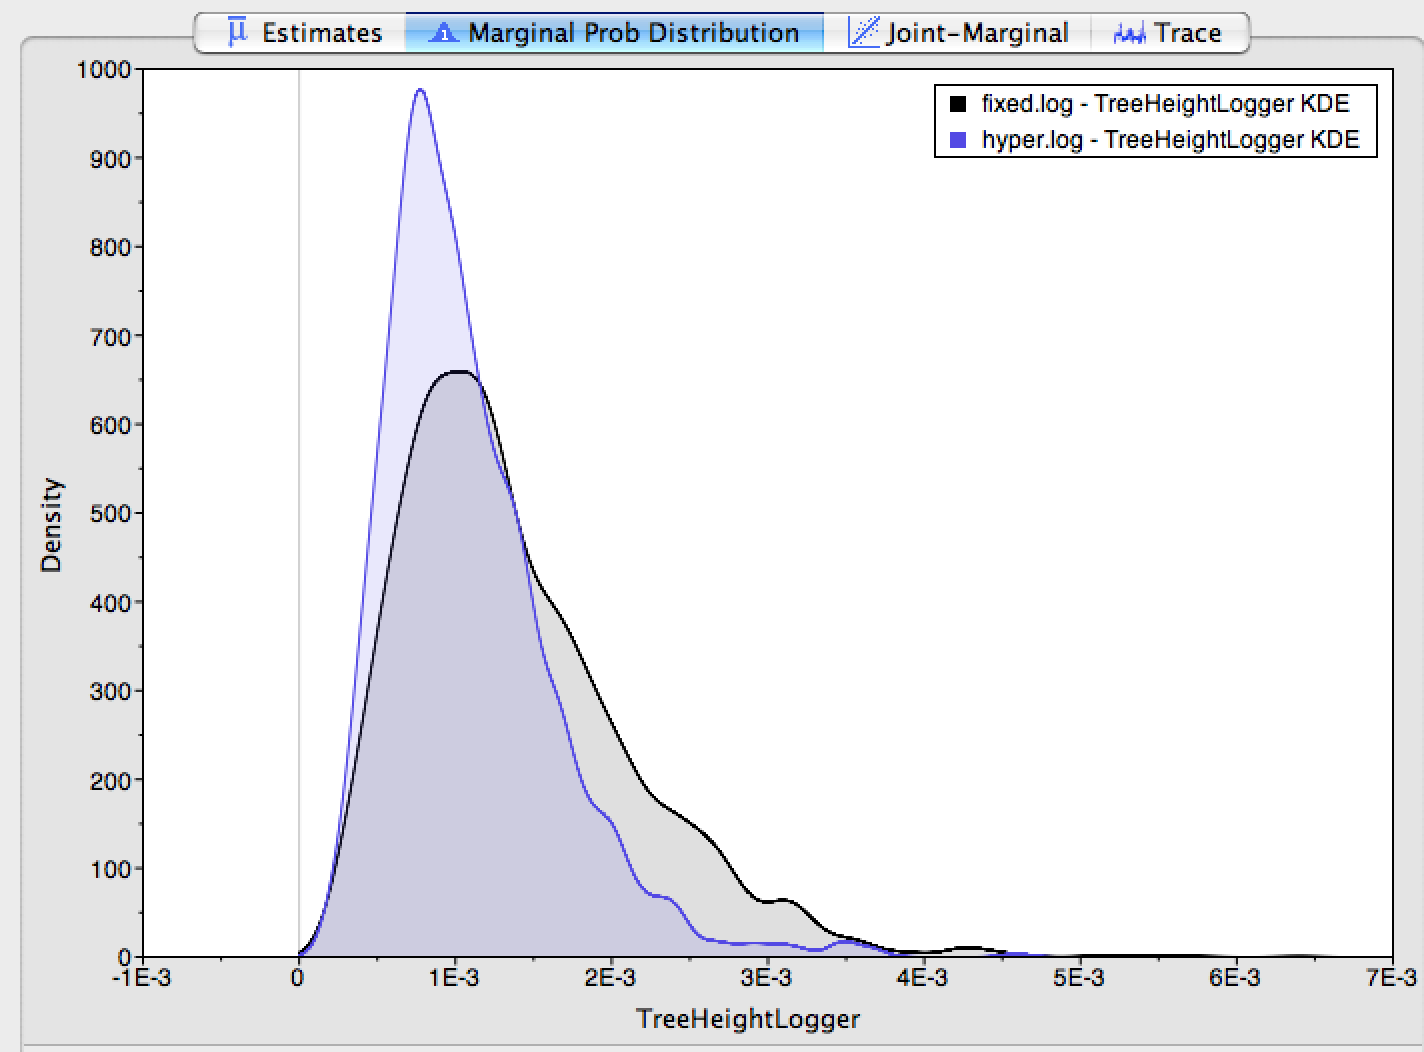
\includegraphics[width=0.8\textwidth]{figures/lambda_comparision.png}}
    \caption{Tree height comparison of analyses using a fixed lambda (lambda = 5) versus a hyperprior on lambda (gamma distribution with mean = 4). The plot shows the marginal probability distributions superimposed for the two estimates, which overlap broadly suggesting that the estimates are quite similar.}
    \label{fig:lambda_comparison}
\end{figure}  

    
\textit{Setting the expected divergence (theta) prior.} Recall that for a diploid population, theta = 4Nu, where N is the effective population size and u is the per-generation mutation rate. If theta=0.004, you expect to observe 0.4\% variation between two randomly sampled alleles in a population. Another way to think about this is in the expected number of substitutions; ``theta=0.004'' means that for two randomly sampled individuals within a population you expect to observe 4 SNPs in 1,000 bases. In SNAPPER, the gamma prior on theta is parameterised such that the mean is alpha*beta. For example, if alpha=2 and beta = 0.002, the prior mean on theta is 0.004. One way of estimating a reasonable mean for the theta prior is to calculate pairwise sequence divergence among all individuals known to belong to a single species and take the average value as the mean for theta. Higher prior means on theta will favour models with populations grouped together, because they represent an expectation that average divergence within populations is relatively high. 
You can select different distributions for the theta prior in the \textbf{Priors} panel. If the prior is set to ``Gamma'' (recommended), the mean value of theta is calculated as alpha*beta when using the ShapeScale mode.  Note that in some implementations, the mean of a gamma distribution is calculated as alpha/beta rather than alpha*beta. 
Here we will leave the default prior.

% \begin{framed}
%     In the \textbf{Priors} tab, click on the arrow next to \textbf{snapperCoalescenceRate} to open the prior details and set \textbf{alpha} to \textbf{100} and \textbf{beta} to \textbf{0.01}.
%     The prior set up should look like Figure \ref{fig:beauti-prior2}.
% \end{framed}

% \begin{figure}[htbp]
%     \centering
%     \fbox{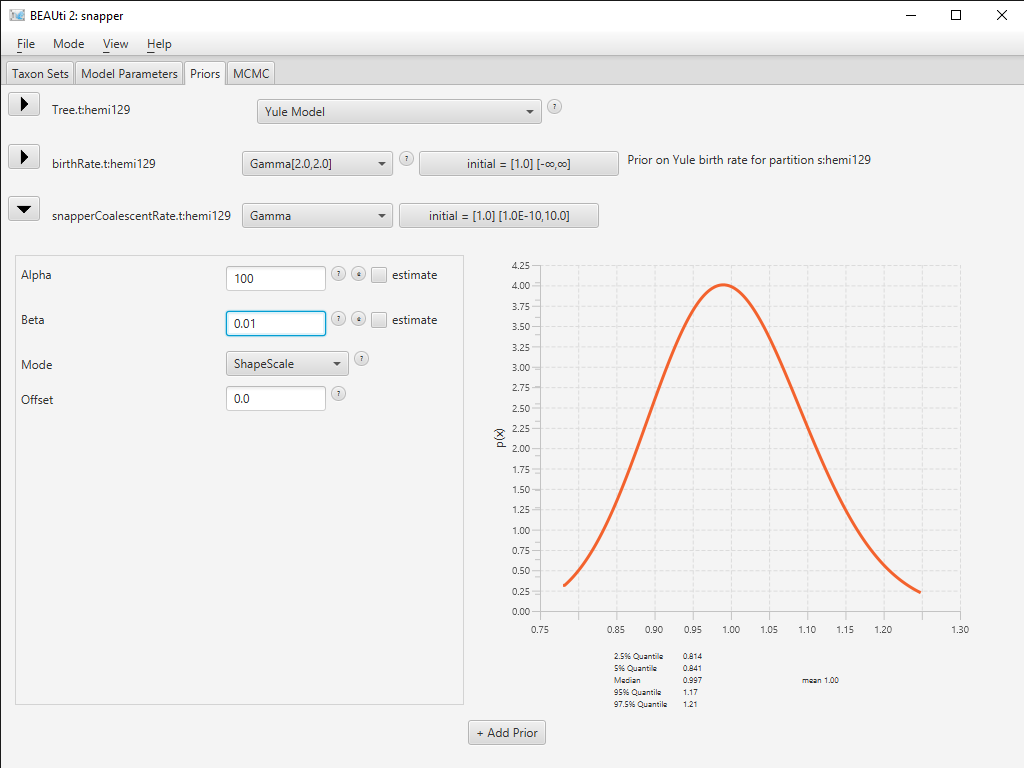
\includegraphics[width=0.8\textwidth]{figures/beauti-prior2.png}}
%     \caption{The prior settings for the coalescence rate.}
%     \label{fig:beauti-prior2}
% \end{figure}  


\subsubsection{Specify MCMC settings and generate the XML file.}

The last step is to configure some run and logging options.

\begin{framed}
    Next, move to the \textbf{MCMC} tab. 
    Change the following settings:
    \begin{itemize}[noitemsep]
        \item \texttt{Chain Length:} \textbf{1000}
        \item \texttt{Store Every:} \textbf{10}
        \item \texttt{tracelog:Log Every:} \textbf{10}
        \item \texttt{treelog:Log Every:} \textbf{10}
    \end{itemize}
    We leave all the remaining options at their default values (Figure~\ref{fig:beauti-mcmc}).
\end{framed}

Note that these MCMC values are way too low, and a thorough analysis requires much more computational time. 
The MCMC run times are intentionally kept short in this tutorial. These short analyses should run in approximately 2 -- 4 minutes depending
on the number of processors available on your computer.  
Thorough analyses of the full data take 2 -- 6 days, depending on the number of species in the model, and generally require at least 100,000 generations. Running multiple independent analyses using different starting seeds and comparing results is a good way to ensure that the analyses are converging.

\begin{figure}[htbp]
    \centering
    \fbox{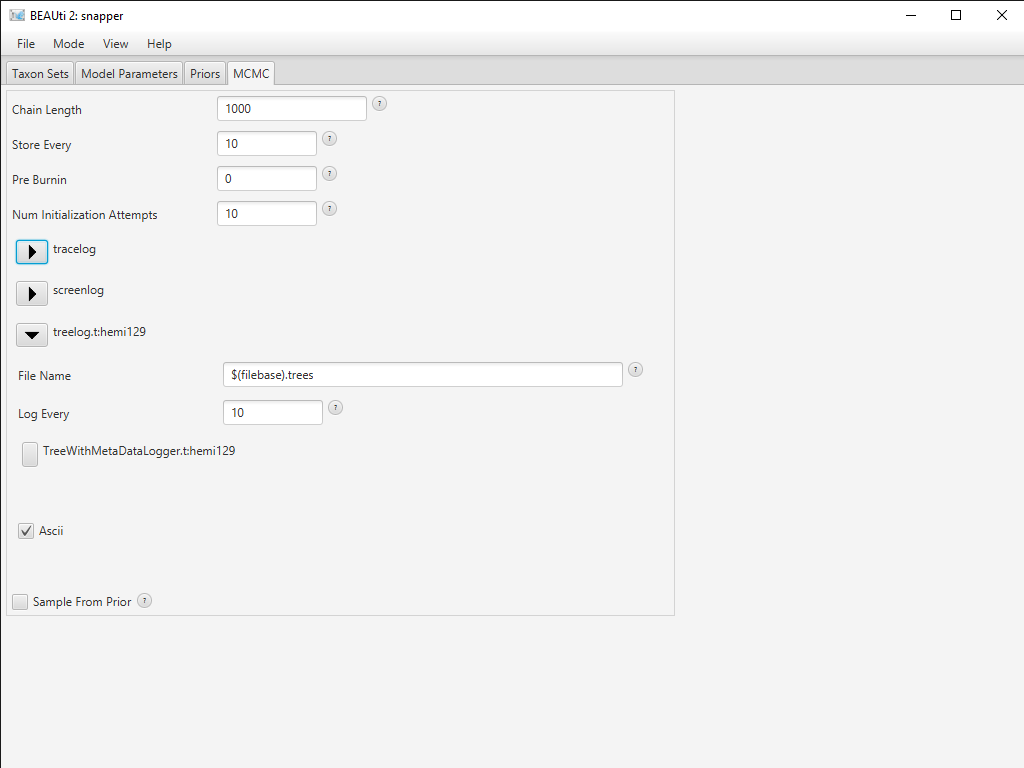
\includegraphics[width=0.75\textwidth]{figures/beauti-mcmc.png}}
    \caption{The MCMC settings.}
    \label{fig:beauti-mcmc}
\end{figure}

\begin{framed}
    Next, save the file using \textbf{File \textgreater{} Save\ldots.} 
    Another subwindow will appear for specifying the name and location for saving the XML file. .
    Name the file \passthrough{\lstinline!runA.xml!} and save it to the \passthrough{\lstinline!SNAPPER-delimitation-tutorial!} folder.\\
\end{framed}


\subsection{Running the analysis in BEAST2}

You can execute the XML file in BEAST2 using the GUI or the command line. If you are using Mac OSX or Windows, you should 
be able to launch the BEAST2 GUI by double clicking on the application icon. 
\begin{framed}
    In the BEAST2 window, click the \textbf{Choose File\ldots} button, and select the XML file you just created (Figure~\ref{fig:beast}). 
    Increase the \textbf{Thread pool size} to speed up your analysis.
    Click the \textbf{Run} button.
\end{framed}
 
Running SNAPPER with multiple threads can increase the speed, but experimenting with the number of threads is required to get the best performance.
The analysis should take about 10 minutes. 

You can also run BEAST2 from the command line. Open the {\bf Terminal} Application and navigate to the folder 
containing your \passthrough{\lstinline!runA.xml!} file. To execute the file, type the following at the command line:

\begin{lstlisting}[language=bash]
/path/to/BEAST2/bin/beast -threads 8 runA.xml
\end{lstlisting}

or

\begin{lstlisting}[language=bash]
beast -threads 8 runA.xml
\end{lstlisting}

if you have already moved the BEAST2 executable to your path. Caution: setting the number of \texttt{threads} beyond the maximum number available on your computer can have serious drawbacks, and you will probably not have enough memory to support all of those separate analyses (i.e. your computer might slow down badly or crash if you use too many threads).

\begin{figure}[htbp]
    \centering
    \fbox{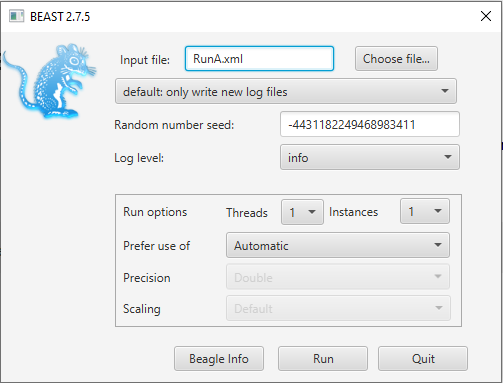
\includegraphics[width=0.5\textwidth]{figures/beast.png}}
    \caption{The BEAST2 GUI window.}
    \label{fig:beast}
\end{figure}

\hypertarget{analyzing-the-output}{%
\subsection{Analyzing the output}\label{analyzing-the-output}}

\hypertarget{output-files}{%
\subsubsection{Output files}\label{output-files}}

Our run has generated 2 different files:

\begin{itemize}
\item \passthrough{\lstinline!RunA.log!} which is the general trace log and stores all parameter values.
\item \passthrough{\lstinline!RunA.trees!} which recorded the sampled trees in Nexus format.
\end{itemize}

By loading the log file into Tracer, we can check that as we expected, we are very far from the convergence of the chain. You can also find two sets of prepared log files in the tutorial, one run with the MCMC parameters set as above (\passthrough{\lstinline!short!}) and one with a longer chain length \passthrough{\lstinline!long!}.

\subsubsection{Summarising the species tree using TreeAnnotator.}

TreeAnnotator will summarize the posterior distribution of species trees and identify the topology with the best posterior support, and summarise the divergence times for each node in the tree.

\begin{framed}
    Launch the \textbf{TreeAnnotator} program.
    Set the \textbf{burnin} value to \textbf{10\%}.
    For the \textbf{Target tree type} field, choose \textbf{Maximum clade credibility tree}.
    For the \textbf{Node heights} field, choose \textbf{Median heights}.
    Select the \textbf{Input Tree File} button and select the file \passthrough{\lstinline!runA.trees!}.
    Select the \textbf{Output File} button and specify the \passthrough{\lstinline!output!} directory and a file name, \passthrough{\lstinline!runA-MCC.tre!}.
    Click \textbf{Run}
\end{framed}

\subsubsection{Visualising the species tree in FigTree.}

We can look at our summary species tree in FigTree.

\begin{framed}
    Launch the FigTree program, and load the \passthrough{\lstinline!runA-MCC.tre!} file you just created with TreeAnnotator.
    Check the \textbf{Branch Labels} option and select \textbf{posterior} for the \textbf{Branch labels}{Display} fields.
    Check the \textbf{Node Bars} option and select \textbf{height\_95\%\_HPD} for the \textbf{Node bars}{Display} field.
\end{framed}

 
You can also get a summary of some tree statistics using the TreeSetAnalyser application, which you can launch from the BEAST app launcher.

\begin{framed}
    First, start the BEAST app-store by selecting the \textbf{File \textgreater{} Launch apps} menu in BEAUti (alternatively, double click the \textbf{AppLauncher} program in the BEAST folder). A window similar to Figure~\ref{fig:appstore} should pop up.
    Select the \textbf{SNAPP tree set analyzer} app, and hit the \textbf{Launch} button. 
\end{framed}

\begin{figure}[htbp]
    \centering
    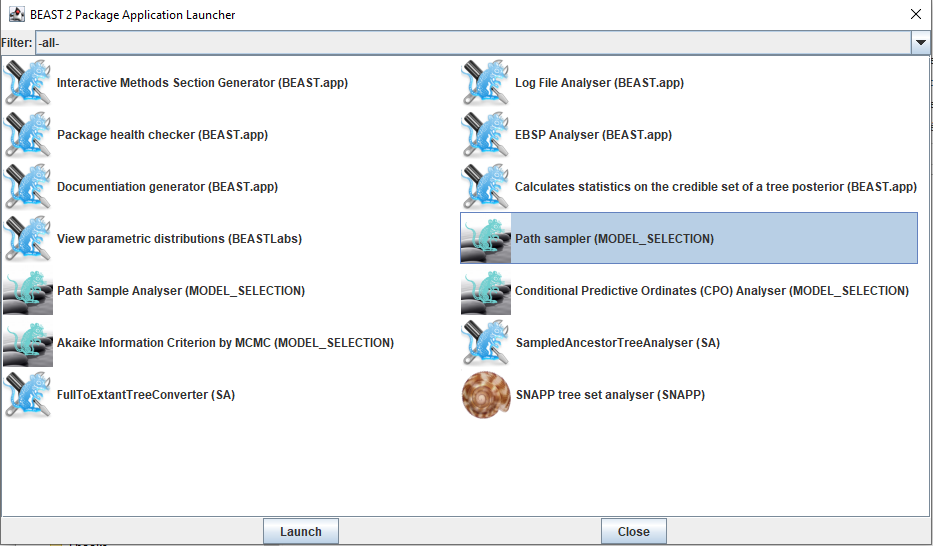
\includegraphics[width=0.6\textwidth]{figures/appstore}
    \caption{BEAST app launcher.}
    \label{fig:appstore}
\end{figure}

A window similar to Figure~\ref{fig:treesetanalyser} will open.

\begin{figure}[htbp]
    \centering
    \fbox{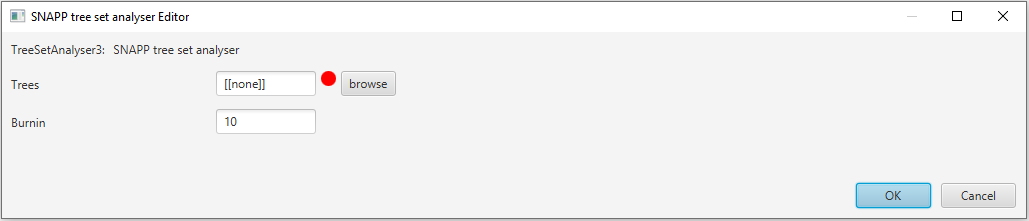
\includegraphics[width=0.75\textwidth]{figures/treesetanalyser.png}}
    \caption{Tree set analyser utility.}
    \label{fig:treesetanalyser}
\end{figure}

\begin{framed}
    Select the \textbf{Browse} button next to the \textbf{Trees} input and select the file \passthrough{\lstinline!runA.trees!}.
    Click on \textbf{OK} to process the file.
\end{framed}

TreeSetAnalyser will compute a summary of the posterior species tree distribution. It will print how many distinct topologies are present in the full distribution and in the 95\% HPD interval, as well as a table of all topologies with their frequency in the posterior distribution, ranked by highest frequency.


\subsection{Running the path sampling analysis with BEAST2}

Species delimitation using SNPs requires marginal likelihood estimation. There are two ways to set up this analysis; through a GUI, and by editing the XML. The GUI is more convenient but makes it a bit harder to transfer the analysis to a cluster, and since path sampling analyses are typically very computational intensive, it often makes sense to run them on a cluster.

\subsubsection{Setting up for marginal likelihood estimation (GUI)}

In this subsubsection, we explain how to set up the analysis using the GUI.

\begin{framed}
    As before, start the BEAST app-store by selecting the \textbf{File \textgreater{} Launch apps} menu in BEAUti (alternatively, double click the \textbf{AppLauncher} program in the BEAST folder). A window similar to Figure~\ref{fig:appstore} should pop up.
    Select the \textbf{Path sampler} app, and hit the \textbf{Launch} button.
\end{framed}

A new window opens with the GUI for path sampling/stepping stone analysis, similar to Figure~\ref{fig:pathsampler}. 

If you prefer to start the app from the command line, you can use the following in a terminal:

\begin{lstlisting}[language=bash]
    /path/to/BEAST2/bin/applauncher PathSampler
\end{lstlisting}


\begin{framed}
    Select the file \passthrough{\lstinline!RunA.xml!} you just set up in BEAUti, and change the following settings:
    \begin{itemize}
        \item \texttt{alpha:} \textbf{0.3}
        \item \texttt{chainLength:} \textbf{1000}
        \item \texttt{burnInPercentage:} \textbf{0}
        \item \texttt{preBurnin:} \textbf{0}
        %\item \texttt{nrOfsubsubsections:} \textbf{24}
    \end{itemize}
    The \textbf{rootdir} option indicates where the run and output files will be placed. Change it to the tutorial folder.
    Note that checking the \textbf{Delete Old Logs} will delete any previous log files in the root directory, so check it only if you are overwriting an old analysis.
\end{framed}

The result should look as indicated in Figure~\ref{fig:pathsampler}.

\begin{figure}[htbp]
    \centering
    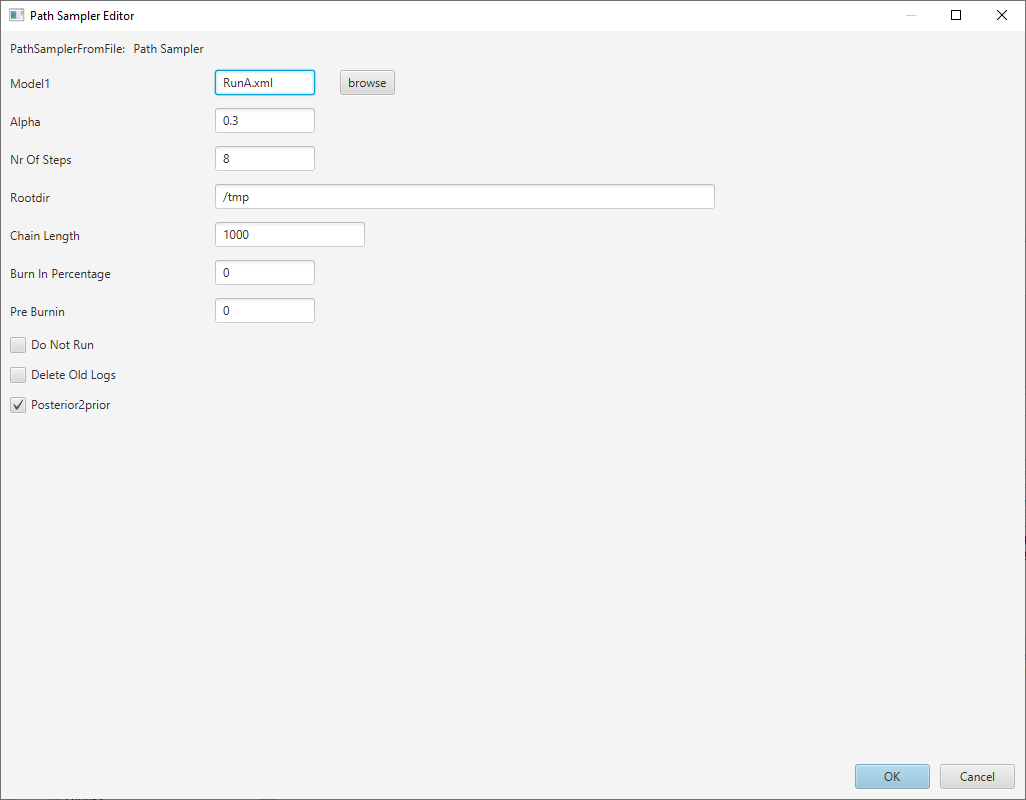
\includegraphics[width=0.7\textwidth]{figures/pathsampler}
    \caption{GUI for path sampling/stepping stone analysis.}
    \label{fig:pathsampler}
\end{figure}

\begin{framed}
    Click on \textbf{OK} to start the analysis.
\end{framed}

The analysis will take a few minutes (it may look like nothing is happening at the beginning). The output will be printed to the application window.
    

\subsubsection{ Editing the XML file for marginal likelihood estimation.}
 
You can also edit the XML file directly to prepare it for path sampling analysis. Detailed instructions for setting up
marginal likelihood estimation using path sampling are provided at the \href{http://www.beast2.org/tutorials}{BEAST2 website}. The procedure involves (1) typing in some short codes in a few places, (2) replacing some words, and (3) copying and pasting some sections around. Specific instructions are below:
 
Open your XML file in a text editor. Search and replace the opening run statement (located about half way through the file) with an mcmc statement by changing {\bf ``<run ...>''} into {\bf ``<mcmc ...>''.} Next, type a new closing mcmc statement, {\bf ``</mcmc>''}, just before the closing run statement, {\bf ``</run>''}, located at the end of the file.

Now you are ready to insert the path sampling commands. You will need to insert the following block of text into your XML file immediately above the opening ``<mcmc ...>''' element:

\begin{lstlisting}[language=XML]
    <run spec='beast.inference.PathSampler' chainLength="1000" alpha='0.3'
    rootdir='/your/path/goes/here/' burnInPercentage='0' preBurnin="0"
    deleteOldLogs='true' nrOfsubsubsections='24'>
\end{lstlisting}

You can then save the XML, then run the analysis by using the following command in the folder where you saved the file.

\begin{lstlisting}[language=bash]
    /path/to/BEAST2/bin/beast path_sampling_runA.xml
\end{lstlisting}

{\bf Important:} If you copy and paste this section into your XML file, be sure to check that the symbols paste correctly. The quote symbols (`` ` ' ") don't copy as they should, and these will cause problems. Also, make sure that the root directory path (rootdir) exists on your computer.

\subsubsection{Parameters of the analysis}

The path sampling parameters that you just entered (either through the GUI or in the XML) are as follows:

\begin{itemize}[noitemsep]
   \item \texttt{chainLength:} MCMC sample length for each path sampling subsubsection.
   \item \texttt{alpha:} parameter used to space out path sampling subsubsections.
   \item \texttt{rootdir:} directory for storing output. Be sure that the folder exists before starting the run.
   \item \texttt{burnInPercentage:} burn-In percentage used for analyzing the log files.
   \item \texttt{preBurnin:} number of samples that are discarded for the first subsubsection, but not the others.
   \item \texttt{deleteOldLogs:} delete existing log files from rootdir
  \item \texttt{nrOfsubsubsections:} the number of path sampling subsubsections to use
\end{itemize}

Note that these path sampling parameters are way to low, and a thorough analysis requires much more computational time. Stable marginal likelihood estimates usually require at least 48 subsubsections (sometimes 100), chainLength = 100,000 (sometimes 1,000,000), and preBurnin=10,000 (sometimes 100,000). The MCMC run times are 
intentionally kept short in this tutorial to obtain quick (but meaningless) results. The run time on a MacBook Pro 2.3GHz i7 processor with 16GB of memory is approximately 2.5 minutes, and this is running 8 concurrent subsubsections (= 8 threads). Increasing the number of threads will speed up the analysis by running more concurrent path sampling subsubsections, but this requires more memory (this analysis uses about 12GB of memory). For large-scale analyses, many users find that they run out of memory before processors.


\subsection{Inspecting path sampling results}

\subsubsection{Inspecting path sampling results.}

At the end of your analysis, the path sampling results will be displayed on the screen. An example (from the GUI) is shown in Figure~\ref{fig:beast-output}. 
Each row shows the results from one path sampling subsubsection. The example in Figure~\ref{fig:beast-output} shows the results from a path sampling analysis with 24 subsubsections. You will use the value after "marginal L estimate" to compare models. 

\begin{figure}[htbp]
    \centering
    \fbox{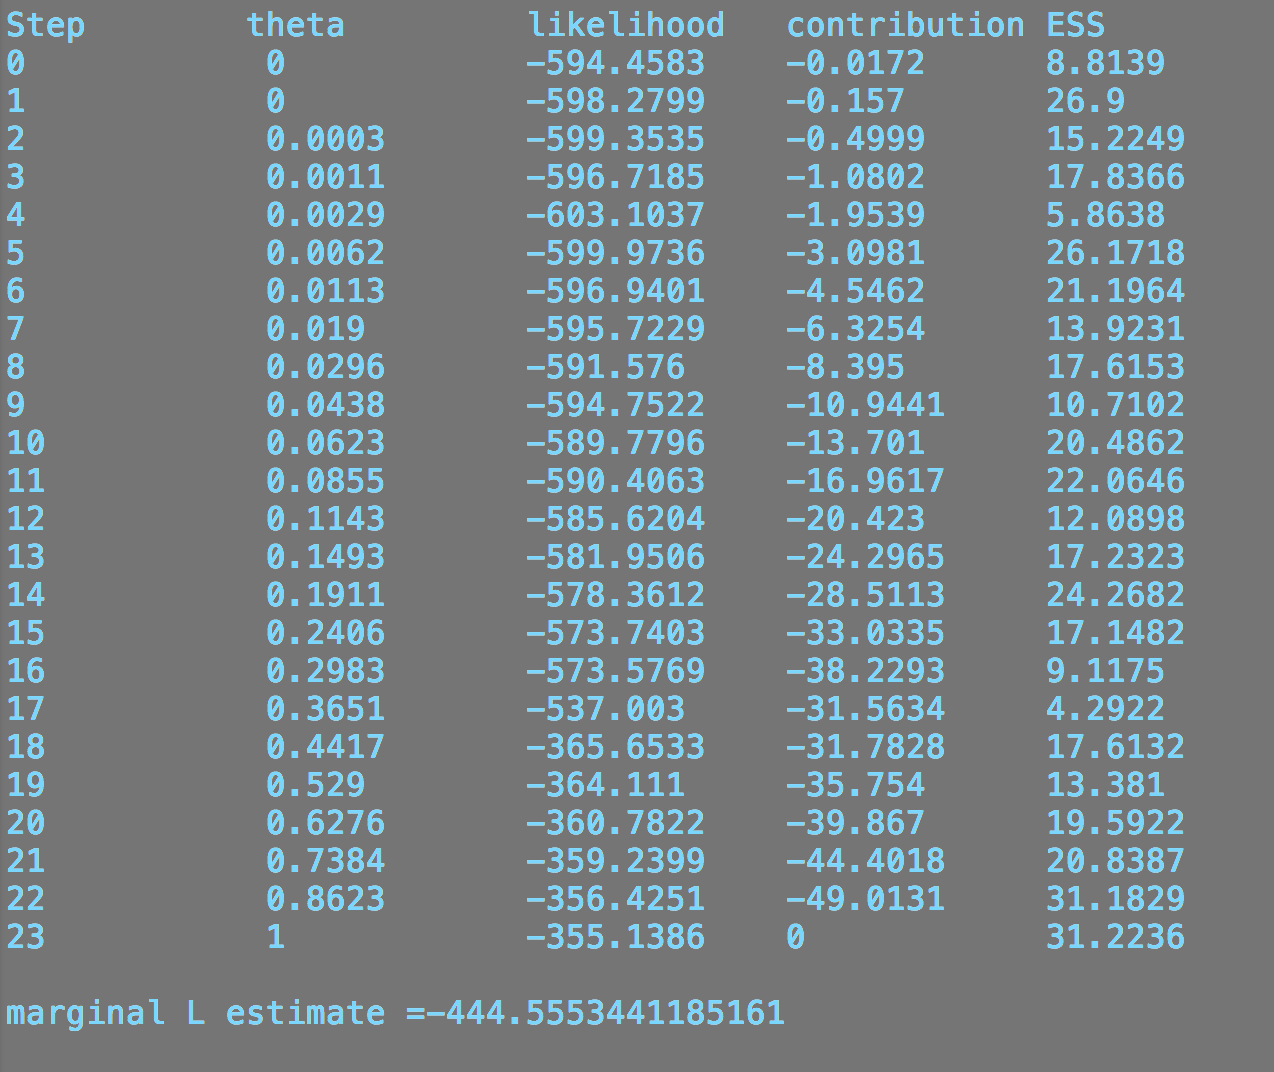
\includegraphics[width=0.5\textwidth]{figures/beast-output.png}}
    \caption{The path sampling output at the end of the analysis.}
    \label{fig:beast-output}
\end{figure}

Note that when conducting path sampling, SNAPPER generates a posterior distribution of trees for each path sampling step. This means we could have skipped the step earlier where we ran \passthrough{\lstinline!runA.xml!} like a regular analysis, and used the output of the path sampling analysis directly instead. You will typically only want to summarize the tree file in the folder corresponding to theta=1, since the other folders contain trees that were estimated with modified likelihoods. Check the SNAPPER screen output to verify which path sampling subsubsection corresponds to theta=1 (this changes with different versions of SNAPPER).


\subsection{Comparing with other species delimitation models}

\subsubsection{Setting up new XML files for species delimitation.}

Now that you have one XML file up and running it is easy to make new XML files for each species delimitation model.

To prepare a new file for species delimitation, make a few slight modifications to the existing \passthrough{\lstinline!runA.xml!} file:
\begin{enumerate}[noitemsep] 
    \item save a copy of the xml file as \passthrough{\lstinline!runB.xml!}, 
    \item change the file logging names in the xml file to \textbf{runB.log} and \textbf{runB.trees} so that you don't accidentally overwrite any of your previous results, 
    \item change the species assignments listed in the  {\bf ``stateDistribution''} element. This last part requires changing the number and/or composition of taxonset features. Each taxonset begins with {\bf ``<taxonset ...>''} and ends with {\bf ``</taxonset>''} (Figure~\ref{fig:beast-taxon-set}). To lump species, simply combine the taxon names into a single taxonset feature. To split a species, simple create a new taxonset containing the appropriate taxon names. To reassign a taxon to another species you can cut and paste the taxon to a different taxonset.
    \item (if you are running directly from the XML instead of using the GUI) edit the path sampling root directory so the output is not overwritten.
\end{enumerate}

XML files containing the species assignments shown in Figure \ref{fig:map} are provided with this tutorial (in the \passthrough{\lstinline!xml!} folder). You don't need to run them, but you can open them in a text editor to see what changes have been made to the species assignments.

\begin{figure}[htbp]
    \centering
    \fbox{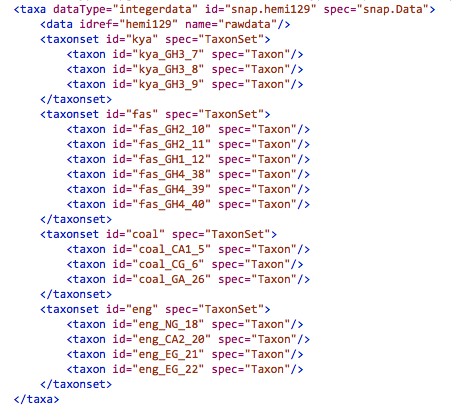
\includegraphics[width=0.5\textwidth]{figures/beast-taxon-set.png}}
    \caption{Example of the taxonset features in the XML file (reduced number of samples to fit on screen, the ready to run XML files for this tutorial contain more samples).}
    \label{fig:beast-taxon-set}
\end{figure}


\subsubsection{Comparing species delimitation models with Bayes factors.}

After you run each of the alternative species delimitation models you can rank them by their marginal likelihood estimate (MLE). You 
can also calculate Bayes factors to compare the models. 
The Bayes factor (BF) is a model selection tool that is simple and well suited for the purposes of comparing species delimitation models. 
Calculating the BF between models is simple. To do so, simply subtract the MLE values for two models, and then multiply the difference by two (BF = 2 x (model1 - model2). A positive BF value indicates support in favour of model 1. A negative BF value indicates support in favour of model 2. 

The strength of support from BF comparisons of competing models can be evaluated using the framework of \cite{kass95}. 
The BF scale is as follows: 0 < BF < 2 is not worth more than a bare mention, 2 < BF < 6 is positive evidence, 6 < BF < 10 is strong support, and BF > 10 is decisive.

The results for the seven gecko models are provided in Table \ref{tab:model_select}. The model that lumps the western forests into one species and splits \textit{eniangii} into two (runS) is the top-ranked model. It has the largest MLE value, and it is supported in favor of the current taxonomy model (runA). The BF in support for model S is decisive compared to model A. It is important to emphasise that these results are \textit{tragically deficient} in terms of the MCMC analysis. Much, much longer runs are required to obtain correct results. 

\begin{table}[ht]
    \tabcolsep=0.2cm
    \begin{center}
    \begin{tabular}{l c c c c } 
    \hline     
    Model 	&	 Species 	&	 MLE 	&	 BF 	&	 Rank\\\hline
    runA     current taxonomy   	&	4	&	-2517.7	&	   -   	&	   2\\
    runB     lump western forests   	&	3	&	-2527.1	&	19.4	&	   5\\
    runC     lump central forests   	&	3	&	-2535.1	&	35.4	&	   6\\
    runD     lump western \&  central forest	&	2	&	-2544.2	&	53.96	&	   7\\
    runE     split \textit{fasciatus}   	&	5	&	-2525.4	&	16.2	&	   4\\
    runF     split \textit{eniangii}    	&	5	&	-2518.3	&	2	&	   3\\
    runG     reassign Bioko Island  	&	4	&	-3348.5	&	1662.2	&	   8\\
    runS    lump western and split \textit{eniangii}    	&	4	&	-2170.4	&	-693.76	&	   1\\
    \end{tabular}\\
    \end{center}
    \caption{Path sampling results for the seven species delimitation models shown in Figure \ref{fig:map}. MLE = Marginal likelihood estimate, BF = Bayes factor. All BF calculations are made against the current taxonomy model (runA). Therefore, positive BF values indicate support for the current taxonomy model, and negative BF values indicate support for the alternative model. .}
    \label{tab:model_select}
\end{table}

Note that as we have seen in this tutorial, Bayesian factor delimitation is computationally expensive, and relies on the user to specify species assignments to test. A recent package \textbf{speedemon} proposes a faster method for species delimitation: find more information and a tutorial on the \href{https://github.com/rbouckaert/speedemon}{package website}.

\hypertarget{useful-links}{%
\section{Useful Links}\label{useful-links}}

\begin{itemize}
\item
  \href{http://www.beast2.org/book.html}{Bayesian Evolutionary Analysis with BEAST 2} \citep{BEAST2book2014}
\item
  BEAST 2 website and documentation: \url{http://www.beast2.org/}
\item
  BEAST 1 website and documentation: \url{http://beast.bio.ed.ac.uk}
\item
  Join the BEAST user discussion:
  \url{http://groups.google.com/group/beast-users} \clearpage
\end{itemize}

\hypertarget{relevant-references}{%
}

\clearpage

%%%%%%%%%%%%%%%%%%%%%%%
% Tutorial disclaimer %
%%%%%%%%%%%%%%%%%%%%%%%
% Please do not change the license
% Add the author names and relevant links
% Add any other aknowledgments here
\href{http://creativecommons.org/licenses/by/4.0/}{
\includegraphics[scale=0.8]{figures/ccby.pdf}} This tutorial was originally written by Adam Leaché and Remco Bouckaert (original version \href{https://github.com/BEAST2-Dev/beast-docs/releases/download/v1.0/snapper-delimitation-tutorial-2021.zip}{on the BEAST2 website}). 
It was adapted by Joëlle Barido-Sottani for \href{https://taming-the-beast.github.io}{Taming the BEAST} and is licensed under a \href{http://creativecommons.org/licenses/by/4.0/}{Creative Commons Attribution 4.0 International License}.


%%%%%%%%%%%%%%%%%%%%
% Do NOT edit this %
%%%%%%%%%%%%%%%%%%%%
Version dated: \today



\newpage

%%%%%%%%%%%%%%%%
%  REFERENCES  %
%%%%%%%%%%%%%%%%

\printbibliography[heading=relevref]


\end{document}
